\chapter{微控制器组成实验}

\section{实验内容}

本实验分为三个子实验:

\begin{itemize}
    \item 微指令控制电路
    \item 微指令寄存器电路
    \item 数据寄存器译码控制电路
\end{itemize}

\section{实验原理}

\subsection{微指令控制电路实验}

\begin{figure}[H]
\centering
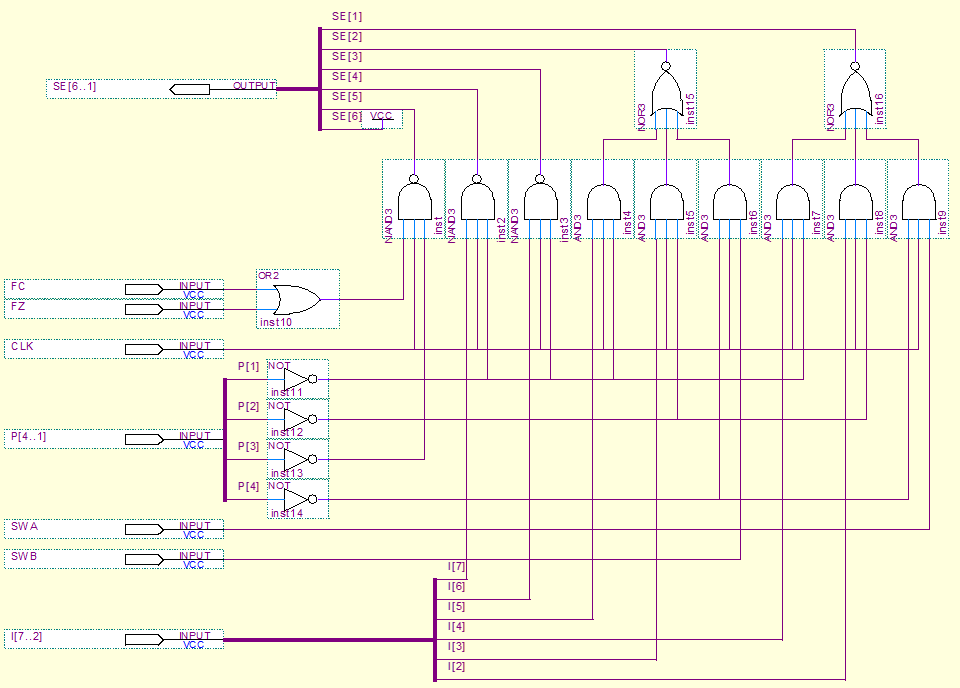
\includegraphics[width=\textwidth]{images/prin5_1.png}
\caption{微指令控制电路}
\label{fig:prin5_1}
\end{figure}

如图\ref{fig:prin5_1},由各种逻辑门电路组合而成。

\subsubsection{输入信号}

\begin{itemize}
    \item FC, FZ
    
    标志信号。
    
    \item CLK
    
    时钟信号。
    
    \item P[4..1]
    
    分支控制信号,4 位。
    
    重置信号,连续节拍发生器的开关。
    
    \item SWA, SWB
    
    控制台控制信号。
    
    \item I[7..2]
    
    指令数据,6 位。
    
\end{itemize} 

\subsubsection{输出信号}

\begin{itemize}
    \item SE[6..1]
    
    输出地址控制信号,6 位。
    
\end{itemize}

\subsection{微指令寄存器电路}

\begin{figure}[H]
\centering
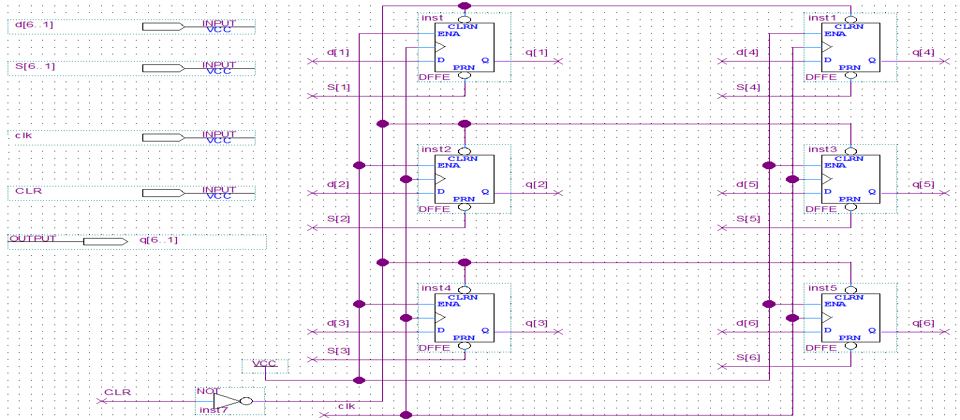
\includegraphics[width=\textwidth]{images/prin5_2.png}
\caption{微指令寄存器电路}
\label{fig:prin5_2}
\end{figure}

如图\ref{fig:prin5_2},由六个 D 触发器、一个非门,形成一个 6 位寄存器,用于寄存微指令控制电路输出的 6 位 SE 地址信号。

\subsubsection{输入信号}

\begin{itemize}
    \item S[6..1]
    
    地址总线信号,6 位。
    
    来自微指令控制电路的输出。
    
    \item clk
    
    时钟信号,每个正脉冲更新所有 D 触发器的输出。
    
    \item CLR
    
    控制信号,控制所有 D 触发器的清空。0: 清空,1: 不清空。
    
    \item d[6..1]
    
    数据信号,D 触发器的默认值数据,6 位。
    
    可通过这个数据信号设置地址掩码(mask code)。
    
\end{itemize} 

\subsubsection{输出信号}

\begin{itemize}
    \item q[6..1]
    
    输出地址信号,6 位。
    
\end{itemize}

\subsection{数据寄存器译码控制电路}


\begin{figure}[H]
\centering
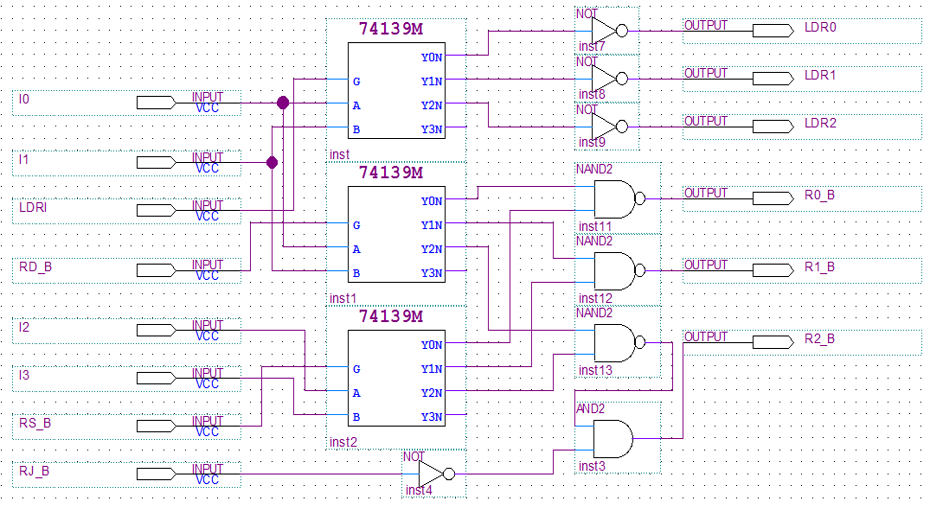
\includegraphics[width=\textwidth]{images/prin5_3.png}
\caption{数据寄存器译码控制电路}
\label{fig:prin5_3}
\end{figure}

如图\ref{fig:prin5_3},由三个 74139M 二四译码器、若干逻辑门组成,形成一个译码电路。

\subsubsection{输入信号}

\begin{itemize}
    \item I0, I1, I2, I3, LDRI, RD\_B, RS\_B, RJ\_B
    
    不可描述的谜之输入信号。
    
\end{itemize} 

\subsubsection{输出信号}

\begin{itemize}
    \item LDR0, LDR1, LDR2, R0\_B, R1\_B, R2\_B
    
    不可描述的谜之输出信号。
    
\end{itemize}

\section{实验任务与实验步骤}

\subsection{微指令控制电路}

\begin{enumerate}
    \item 按照原理图 \ref{fig:prin5_1} 连接电路图,然后编译。
    \item 将输入输出器件绑定到对应的引脚上,然后重新编译。
    
    
    \begin{table}[H]
        \centering
        \begin{tabular}{|c|c|c|}
            \hline
            名称 & 引脚号 & 备注 \\
            \hline
            CLK & 173 & Key 8 \\
            \hline
            I[2] & 233 & Key 1 \\
            \hline
            I[3] & 234 & Key 1 \\
            \hline
            I[4] & 235 & Key 1 \\
            \hline
            I[5] & 236 & Key 1 \\
            \hline
            I[6] & 237 & Key 2 \\
            \hline
            I[7] & 238 & Key 2 \\
            \hline
            FC & 239 & Key 2 \\
            \hline
            FZ & 240 & Key 2 \\
            \hline
            P[1] & 1 & Key 3 \\
            \hline
            P[2] & 2 & Key 3 \\
            \hline
            P[3] & 3 & Key 3 \\
            \hline
            P[4] & 4 & Key 3 \\
            \hline
            SWA & 6 & Key 4 \\
            \hline
            SWB & 7 & Key 4 \\
            \hline
            SE[1] & 13 & 数码 5 \\
            \hline
            SE[2] & 14 & 数码 5 \\
            \hline
            SE[3] & 15 & 数码 5 \\
            \hline
            SE[4] & 16 & 数码 5 \\
            \hline
            SE[5] & 17 & 数码 6 \\
            \hline
            SE[6] & 18 & 数码 6 \\
            \hline
        \end{tabular}
        \caption{微指令控制电路实验:引脚表}
        \label{tab:pin5_1}
    \end{table}
    
    \item 下载到实验设备上。
    \item 调整为工作模式 1。
    \item 观察实验现象。
    
    \begin{itemize}
        \item Key 1, 2 (数码 1, 2)
        
        输入 I 数据 (低 6 位)
        
        输入 FC (最高位)
        
        输入 FZ (次高位)
        
        \item Key 3 (数码 3)
        
        输入 P 数据,4 位全有效。
        
        \item Key 4 (数码 4)
        
        输入 SWA (最低位)
        
        输入 SWB (次低位)
        
        \item Key 8 (D16)
        
        时钟信号。
        
        \item 数码 5, 6
        
        输出的 SE 信号,低 6 位有效。
        
    \end{itemize}
    \item 绘制仿真波形图。
\end{enumerate}

\subsection{微指令寄存器电路}

\begin{enumerate}
    \item 按照原理图 \ref{fig:prin5_2} 连接电路图,然后编译。
    \item 将输入输出器件绑定到对应的引脚上,然后重新编译。
    
    \begin{table}[H]
        \centering
        \begin{tabular}{|c|c|c|}
            \hline
            名称 & 引脚号 & 备注 \\
            \hline
            CLR & 169 & Key 7 \\
            \hline
            clk & 173 & Key 8 \\
            \hline
            d[1] & 233 & Key 1 \\
            \hline
            d[2] & 234 & Key 1 \\
            \hline
            d[3] & 235 & Key 1 \\
            \hline
            d[4] & 236 & Key 1 \\
            \hline
            d[5] & 237 & Key 2 \\
            \hline
            d[6] & 238 & Key 2 \\
            \hline
            S[1] & 1 & Key 3 \\
            \hline
            S[2] & 2 & Key 3 \\
            \hline
            S[3] & 3 & Key 3 \\
            \hline
            S[4] & 4 & Key 3 \\
            \hline
            S[5] & 6 & Key 4 \\
            \hline
            S[6] & 7 & Key 4 \\
            \hline
            q[1] & 21 & 数码 7 \\
            \hline
            q[2] & 41 & 数码 7 \\
            \hline
            q[3] & 128 & 数码 7 \\
            \hline
            q[4] & 132 & 数码 7 \\
            \hline
            q[5] & 133 & 数码 8 \\
            \hline
            q[6] & 134 & 数码 8 \\
            \hline
        \end{tabular}
        \caption{微指令寄存器电路实验:引脚表}
        \label{tab:pin5_2}
    \end{table}
    
    \item 下载到实验设备上。
    \item 调整为工作模式 1。
    \item 观察实验现象。
    
    \begin{itemize}
        \item Key 1, 2 (数码 1, 2)
        
        输入 d 数据,低 6 位有效。
        
        \item Key 3, 4 (数码 3, 4)
        
        输入 S 数据,低 6 位有效。
        
        \item Key 7 (D15)
        
        寄存器清空信号,低电平有效。
        
        \item Key 8 (D16)
        
        时钟信号。
        
        \item 数码 7, 8
        
        输出的 q 数据,低 6 位有效。
        
    \end{itemize}
    \item 绘制仿真波形图。
\end{enumerate}

\subsection{数据寄存器译码控制电路}

\begin{enumerate}
    \item 按照原理图 \ref{fig:prin5_3} 连接电路图,然后编译。
    \item 将输入输出器件绑定到对应的引脚上,然后重新编译。
    
    \begin{table}[H]
        \centering
        \begin{tabular}{|c|c|c|}
            \hline
            名称 & 引脚号 & 备注 \\
            \hline
            I0 & 233 & Key 1 (D9) \\
            \hline
            I1 & 234 & Key 2 (D10) \\
            \hline
            I2 & 235 & Key 3 (D11) \\
            \hline
            I3 & 236 & Key 4 (D12) \\
            \hline
            LDRI & 237 & Key 5 (D13) \\
            \hline
            I2 & 238 & Key 6 (D14) \\
            \hline
            I3 & 239 & Key 7 (D15) \\
            \hline
            LDRI & 240 & Key 8 (D16) \\
            \hline
            LDR0 & 1 & D1 \\
            \hline
            LDR1 & 2 & D2 \\
            \hline
            LDR2 & 3 & D3 \\
            \hline
            R0\_B & 7 & D6 \\
            \hline
            R1\_B & 8 & D7 \\
            \hline
            R2\_B & 12 & D8 \\
            \hline
        \end{tabular}
        \caption{数据寄存器译码控制电路实验:引脚表}
        \label{tab:pin5_3}
    \end{table}
    
    \item 下载到实验设备上。
    \item 调整为工作模式 5。
    \item 观察实验现象。
    
    参照引脚表 \ref{tab:pin5_3},按键 1 - 8,观察 LED 灯 1 - 3, 6 - 16 的值。
    
    \item 绘制仿真波形图。
\end{enumerate}

\section{实验结果分析}

\subsection{实验电路图}

根据原理图 \ref{fig:prin5_1} 绘制实验电路图 \ref{fig:bdf5_1}。

\begin{figure}[H]
\centering
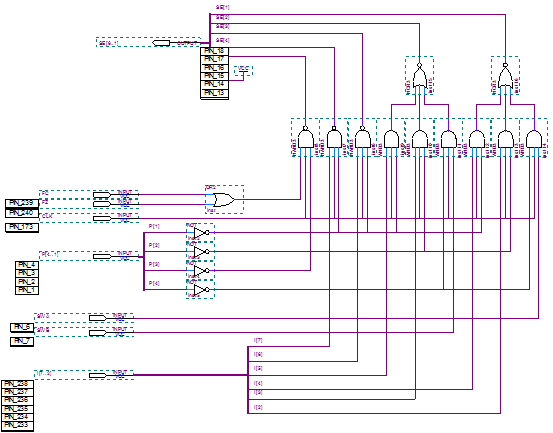
\includegraphics[width=\textwidth]{images/bdf5_1.png}
\caption{微指令控制电路图}
\label{fig:bdf5_1}
\end{figure}

根据原理图 \ref{fig:prin5_2} 绘制实验电路图 \ref{fig:bdf5_2}。

\begin{figure}[H]
\centering
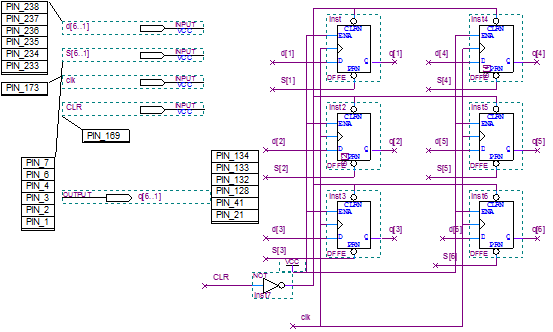
\includegraphics[width=\textwidth]{images/bdf5_2.png}
\caption{微指令寄存器电路图}
\label{fig:bdf5_2}
\end{figure}

根据原理图 \ref{fig:prin5_3} 绘制实验电路图 \ref{fig:bdf5_3}。

\begin{figure}[H]
\centering
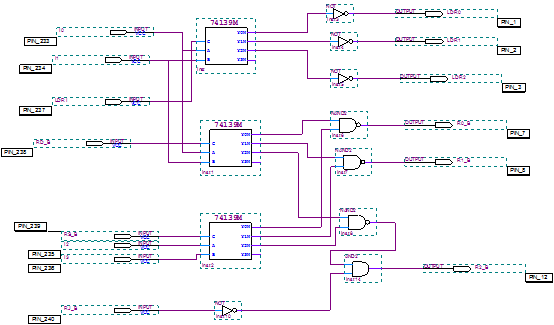
\includegraphics[width=\textwidth]{images/bdf5_3.png}
\caption{数据寄存器译码控制电路图}
\label{fig:bdf5_3}
\end{figure}

\subsection{仿真波形图}

利用 Quartus II 产生仿真波形图 \ref{fig:wave5_1}。

\begin{figure}[H]
\centering
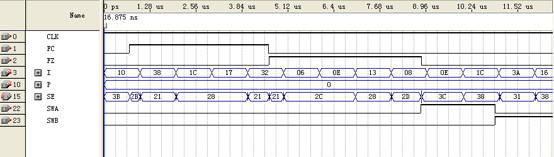
\includegraphics[width=\textwidth]{images/wave5_1.png}
\caption{微指令控制电路 仿真波形图}
\label{fig:wave5_1}
\end{figure}

利用 Quartus II 产生仿真波形图 \ref{fig:wave5_2}。

\begin{figure}[H]
\centering
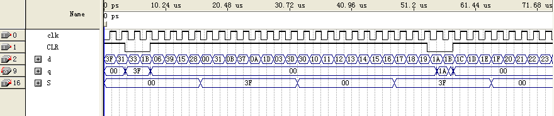
\includegraphics[width=\textwidth]{images/wave5_2.png}
\caption{微指令寄存器电路 仿真波形图}
\label{fig:wave5_2}
\end{figure}

利用 Quartus II 产生仿真波形图 \ref{fig:wave5_3}。

\begin{figure}[H]
\centering
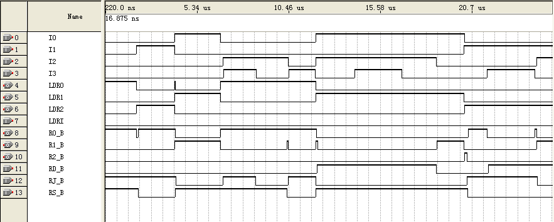
\includegraphics[width=\textwidth]{images/wave5_3.png}
\caption{数据寄存器译码控制电路 仿真波形图}
\label{fig:wave5_3}
\end{figure}

\subsection{思考题}

\begin{enumerate}
    \item 在微指令控制电路中,当 FC 或 FZ 有效时,对其输出 SE[6..1] 有何影响?对微地址寄存器的输出会有何影响?如何实现对程序的控制/转移功能?
    
    \textbf{答}:
    
    讨论 FC 或 FZ 有效时:
    
    \textbf{对输出 SE 的影响:等同于 FC, FZ 直接接地}
    
    首先 FC, FZ 只可能对 SE[5] 有影响,对 SE 其他位无影响(等同于接地)。
    
    且仅当 FC = FZ = 0 时影响 S[5] = 1。
    
    那么当 FC 或 FZ 有效时,其对 SE 无影响。
    
    \textbf{对微地址寄存器的输出的影响:等同于 FC, FZ 直接接地}
    
    微地址寄存器的输入来源于微指令控制电路的输出,由上题得无影响(等同于接地)。

    结束 FC, FZ 的讨论。
    
    \textbf{讨论如何实现程序的控制/转移:输入恰当的 P 值}
    
    P 值是微程序功能码,会被译码成指令。某个 P 对应的是控制/转移指令,就可以实现控制/转移。
    
    \item 说明 P[4..1] 信号分别有效时,对微指令控制电路中输出 SE[6..1] 有何影响?
    
    \textbf{答}:
    
    \begin{itemize}
        \item P[1] = 1 时
        
        \begin{itemize}
            \item 直接影响 SE[3] = SE[4] = 1
            \item 屏蔽了 I[5] 对 SE[2] 的影响
            \item 屏蔽了 I[4] 对 SE[1] 的影响
        \end{itemize}
        
        \item P[2] = 1 时
        
        \begin{itemize}
            \item 屏蔽了 I[3] 对 SE[2] 的影响
            \item 屏蔽了 I[2] 对 SE[1] 的影响            
        \end{itemize}
        
        \item P[3] = 1 时
        
        \begin{itemize}
            \item 直接影响 SE[5] = 1
        \end{itemize}
        
        \item P[4] = 1 时
        
        \begin{itemize}
            \item 屏蔽了 SWB 对 SE[2] 的影响
            \item 屏蔽了 SWA 对 SE[1] 的影响
        \end{itemize}
    \end{itemize}
    
    \item 当控制信号 SWA、SWB 取不同的值时,对微指令控制电路中输出 SE[6..1] 有何影响?
    
    \textbf{答}:
    
    SWA 影响 SE[1], SWB 影响 SE[2],互相独立。
    
    当 SWx = 0 时,能屏蔽 P[4] 对上述对应的 SE[y] 的影响。
    
\end{enumerate}
